\chapter{FUNCIONES DE VARIAS VARIABLES}
%\startcontents
\printchaptertableofcontents

El estudio de las funciones de varias variables constituye un pilar fundamental en el ámbito del Cálculo III, donde se exploran fenómenos matemáticos que implican más de una dimensión. A diferencia del cálculo de una sola variable, donde las funciones dependen únicamente de un parámetro, en el cálculo de varias variables, las funciones pueden depender de dos o más variables independientes. Este capítulo se adentra en la comprensión y análisis de estas funciones, explorando su comportamiento, propiedades y aplicaciones en diversos contextos.

En esencia, una función de varias variables asigna a cada punto en un dominio de dos o más dimensiones un único valor en el espacio real. Este enfoque multifacético permite modelar y comprender una amplia gama de fenómenos físicos, económicos y científicos, desde la trayectoria de un proyectil en el espacio hasta la distribución de temperatura en un sólido tridimensional.

La comprensión de las funciones de varias variables requiere el dominio de conceptos clave, entre ellos, la noción de dominio y rango, continuidad, derivadas parciales, gradientes, y optimización. A través del análisis de estas herramientas matemáticas, los estudiantes desarrollarán una perspicacia profunda sobre cómo las funciones de varias variables se comportan y cómo pueden ser utilizadas para resolver problemas prácticos.

Este capítulo se estructura para guiar al lector desde los conceptos básicos hasta las aplicaciones avanzadas. Comienza con la definición formal de una función de varias variables, examinando su representación gráfica y sus propiedades fundamentales. A medida que avanzamos, exploramos la diferenciabilidad y la integrabilidad de estas funciones, así como las técnicas para encontrar máximos y mínimos locales y absolutos.

Además, se abordan aplicaciones relevantes en campos como la física, la ingeniería, la economía y las ciencias computacionales, ilustrando cómo las funciones de varias variables se utilizan para modelar situaciones del mundo real y resolver problemas complejos.

\section{Funciones}\index{Funciones}

\begin{definition}
    Una función $f$ de dos variables es una regla que asigna a cada par ordenado de números reales $(x, y)$ de un conjunto $D$, un único número real que se denota con $f(x, y)$. El conjunto $D$ es el dominio de $f$ y su rango es el conjunto de valores que toma $f$, es decir, $\left\{ f(x, y) \mid (x, y) \in D \right\}$.
\end{definition}

A menudo, escribimos $z = f(x, y)$ para hacer explícito el valor que toma $f$ en el punto $(x, y)$. Las variables $x$ y $y$ son variables independientes y $z$ es la variable dependiente [compare lo anterior con la notación $y = f(x)$ para funciones de una variable].
\sideFigure[\label{fig:Funcion_dos_variables}]{
    \centering
    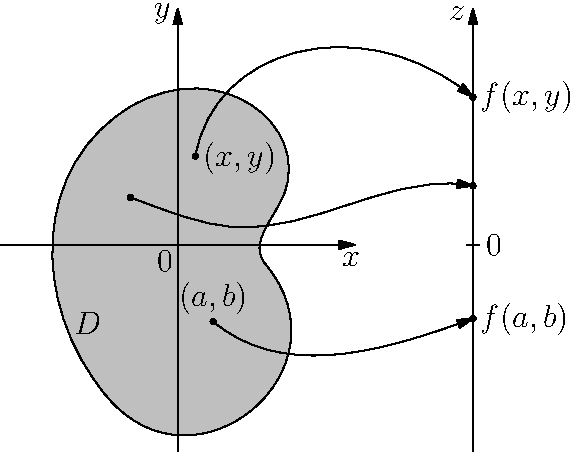
\includegraphics[width=\linewidth]{Images/Capitulo1/Funcion_dos_variables.pdf}
}

Una función de dos variables es una función cuyo dominio es un subconjunto de $\mathbb{R}^2$ y cuyo rango es un subconjunto de $\mathbb{R}$. Una manera de representar tal función es mediante un diagrama de flechas (véase la figura \ref{fig:Funcion_dos_variables}), donde el dominio $D$ se representa como un subconjunto del plano $x y$ y el rango es un conjunto de números sobre una recta real, que se muestra como un eje $z$. Por ejemplo, si $f(x, y)$ representa la temperatura en un punto $(x, y)$ en una placa metálica plana con la forma de $D$, podemos considerar al eje $z$ como un termómetro que va mostrando el registro de temperaturas.

Si una función $f$ está dada por una fórmula y no se especifica dominio alguno, entonces se entiende que el dominio de $f$ será el conjunto de parejas $(x, y)$ para el cual la expresión dada es un número bien definido.

\begin{example}
    Para las siguientes funciones, evalúe $f(3, 2)$ y determine y grafique el dominio.
    \begin{tasks}(2)
        \task $\displaystyle f(x, y) = \frac{\sqrt{x + y + 1}}{x - 1}$
        \task $f(x, y) = x \ln (y^2 - x)$
    \end{tasks}
    \solucion
    \begin{enumerate}[label=\alph*)]
        \item Tenemos que\sideFigure[\label{Fig:Dominio_1}Representación geométrica del dominio de $\displaystyle f(x, y) = \frac{\sqrt{x + y + 1}}{x - 1}$]{
        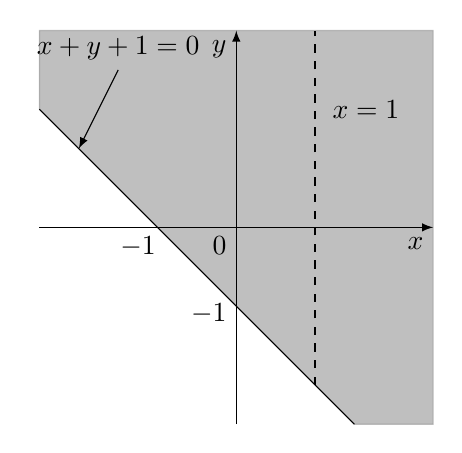
\begin{tikzpicture}
            \filldraw[gray,opacity=0.5] (1.5,-2.5) --(2.5,-2.5) -- (2.5,2.5) -- (-2.5,2.5) -- (-2.5,1.5) -- (1.5,-2.5) -- cycle;
            \draw[-latex] (-2.5,0) -- (2.5,0) node[below left] {$x$};
            \draw[-latex] (0,-2.5) -- (0,2.5) node[below left] {$y$};
            \draw (-2.5,1.5) -- (1.5,-2.5);
            \draw[latex-] (-2,1) -- (-1.5,2) node[above] {$x + y + 1 = 0$};
            \node[below left] at (0,0) {$0$};
            \node[below left] at (-0.9,0) {$-1$};
            \node[left] at (0,-1.1) {$-1$};
            \draw[dash pattern=on 3pt off 3pt] (1,-2) -- (1,2.5);
            \node[right] at (1.1,1.5) {$x = 1$};
        \end{tikzpicture}
        }
        $$f(3, 2) = \frac{\sqrt{3 + 2 + 1}}{3 - 1} = \frac{\sqrt{6}}{2}$$
        La expresión para $f$ tiene sentido si el denominador no es cero y la cantidad dentro del signo de raíz cuadrada es no negativa. Entonces, el dominio de $f$ es
        $$D = \left\{ (x, y) \mid x + y + 1 \geq 0, x \neq 1 \right\}.$$
        La desigualdad $x + y + 1 \geq 0$, o $y \geq -x - 1$, describe los puntos que quedan en o por arriba de la recta $y = -x - 1$, mientras que $x \neq 1$ significa que los puntos sobre la recta $x = 1$ tienen que ser excluidos del dominio. Vea la figura \ref{Fig:Dominio_1}.
        \item Tenemos que\sideFigure[\label{Fig:Dominio_2}Representación geométrica del dominio de $f(x, y) = x \ln (y^2 - x)$]{
        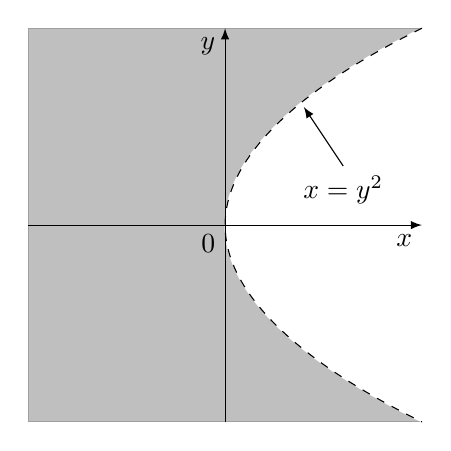
\begin{tikzpicture}
            \filldraw[gray,opacity=0.5] (-2.5,-2.5) rectangle (2.49,2.5);
            \node[below left] at (0,0) {$0$};
            \filldraw[rotate=-90,white] (-2.5,2.5) parabola bend (0,0) (2.5,2.5);
            \draw[rotate=-90,dash pattern=on 3pt off 3pt] (-2.5,2.5) parabola bend (0,0) (2.5,2.5);
            \draw[latex-] (1,1.5) -- (1.5,0.75) node[below] {$x = y^2$};
            \draw[-latex] (-2.5,0) -- (2.5,0) node[below left] {$x$};
            \draw[-latex] (0,-2.5) -- (0,2.5) node[below left] {$y$};
        \end{tikzpicture}
        }
        $$f(3, 2) = 3 \ln (2^2 - 3) = 0.$$
        Puesto que $\ln(y^2 - x)$ se define solo cuando $y^2 - x > 0$, es decir, $x < y^2$, el dominio de $f$ es
        $$D = \left\{ (x, y) \mid x < y^2 \right\}.$$
        Este es el conjunto de puntos a la izquierda de la parábola $x = y^2$. Vea la figura \ref{Fig:Dominio_2}.
    \end{enumerate}
\end{example}

\section{Curvas de nivel}